%%%%%%%%%%%%%%%%%%%%%%%%%%%%%%%%%%%%%%%%%
% Arsclassica Article
% LaTeX Template
% Version 1.1 (10/6/14)
%
% This template has been downloaded from:
% http://www.LaTeXTemplates.com
%
% Original author:
% Lorenzo Pantieri (http://www.lorenzopantieri.net) with extensive modifications by:
% Vel (vel@latextemplates.com)
%
% License:
% CC BY-NC-SA 3.0 (http://creativecommons.org/licenses/by-nc-sa/3.0/)
%
%%%%%%%%%%%%%%%%%%%%%%%%%%%%%%%%%%%%%%%%%

%----------------------------------------------------------------------------------------
%	PACKAGES AND OTHER DOCUMENT CONFIGURATIONS
%----------------------------------------------------------------------------------------

\documentclass[
10pt, % Main document font size
a4paper, % Paper type, use 'letterpaper' for US Letter paper
oneside, % One page layout (no page indentation)
%twoside, % Two page layout (page indentation for binding and different headers)
headinclude,footinclude, % Extra spacing for the header and footer
BCOR5mm, % Binding correction
]{scrartcl}

%%%%%%%%%%%%%%%%%%%%%%%%%%%%%%%%%%%%%%%%%
% Arsclassica Article
% Structure Specification File
%
% This file has been downloaded from:
% http://www.LaTeXTemplates.com
%
% Original author:
% Lorenzo Pantieri (http://www.lorenzopantieri.net) with extensive modifications by:
% Vel (vel@latextemplates.com)
%
% License:
% CC BY-NC-SA 3.0 (http://creativecommons.org/licenses/by-nc-sa/3.0/)
%
%%%%%%%%%%%%%%%%%%%%%%%%%%%%%%%%%%%%%%%%%

%----------------------------------------------------------------------------------------
%	REQUIRED PACKAGES
%----------------------------------------------------------------------------------------

\usepackage[
nochapters, % Turn off chapters since this is an article        
beramono, % Use the Bera Mono font for monospaced text (\texttt)
eulermath,% Use the Euler font for mathematics
pdfspacing, % Makes use of pdftex’ letter spacing capabilities via the microtype package
dottedtoc % Dotted lines leading to the page numbers in the table of contents
]{classicthesis} % The layout is based on the Classic Thesis style

\usepackage{arsclassica} % Modifies the Classic Thesis package

\usepackage[T1]{fontenc} % Use 8-bit encoding that has 256 glyphs

\usepackage[utf8]{inputenc} % Required for including letters with accents

\usepackage{graphicx} % Required for including images
\graphicspath{{Figures/}} % Set the default folder for images

\usepackage{enumitem} % Required for manipulating the whitespace between and within lists

\usepackage{lipsum} % Used for inserting dummy 'Lorem ipsum' text into the template

\usepackage{subfig} % Required for creating figures with multiple parts (subfigures)

\usepackage{amsmath,amssymb,amsthm} % For including math equations, theorems, symbols, etc

\usepackage{varioref} % More descriptive referencing
\usepackage{color}
\usepackage{listings}
\usepackage{setspace}

\usepackage{lscape}


%----------------------------------------------------------------------------------------
%	THEOREM STYLES
%---------------------------------------------------------------------------------------

\theoremstyle{definition} % Define theorem styles here based on the definition style (used for definitions and examples)
\newtheorem{definition}{Definition}

\theoremstyle{plain} % Define theorem styles here based on the plain style (used for theorems, lemmas, propositions)
\newtheorem{theorem}{Theorem}

\theoremstyle{remark} % Define theorem styles here based on the remark style (used for remarks and notes)

%----------------------------------------------------------------------------------------
%	HYPERLINKS
%---------------------------------------------------------------------------------------

\hypersetup{
%draft, % Uncomment to remove all links (useful for printing in black and white)
colorlinks=true, breaklinks=true, bookmarks=true,bookmarksnumbered,
urlcolor=webbrown, linkcolor=RoyalBlue, citecolor=webgreen, % Link colors
pdftitle={}, % PDF title
pdfauthor={\textcopyright}, % PDF Author
pdfsubject={}, % PDF Subject
pdfkeywords={}, % PDF Keywords
pdfcreator={pdfLaTeX}, % PDF Creator
pdfproducer={LaTeX with hyperref and ClassicThesis} % PDF producer
}

\definecolor{Code}{rgb}{0,0,0}
\definecolor{Decorators}{rgb}{0.5,0.5,0.5}
\definecolor{Numbers}{rgb}{0.5,0,0}
\definecolor{MatchingBrackets}{rgb}{0.25,0.5,0.5}
\definecolor{Keywords}{rgb}{0,0,1}
\definecolor{self}{rgb}{0,0,0}
\definecolor{Strings}{rgb}{0,0.63,0}
\definecolor{Comments}{rgb}{0,0.63,1}
\definecolor{Backquotes}{rgb}{0,0,0}
\definecolor{Classname}{rgb}{0,0,0}
\definecolor{FunctionName}{rgb}{0,0,0}
\definecolor{Operators}{rgb}{0,0,0}
\definecolor{Background}{rgb}{0.98,0.98,0.98}

\lstnewenvironment{python}[1][]{
\lstset{
numbers=left,
numberstyle=\footnotesize,
numbersep=1em,
xleftmargin=1em,
framextopmargin=2em,
framexbottommargin=2em,
showspaces=false,
showtabs=false,
showstringspaces=false,
frame=l,
tabsize=4,
% Basic
basicstyle=\ttfamily\small\setstretch{1},
backgroundcolor=\color{Background},
language=Python,
% Comments
commentstyle=\color{Comments}\slshape,
% Strings
stringstyle=\color{Strings},
morecomment=[s][\color{Strings}]{"""}{"""},
morecomment=[s][\color{Strings}]{'''}{'''},
% keywords
morekeywords={import,from,class,def,for,while,if,is,in,elif,else,not,and,or,print,break,continue,return,True,False,None,access,as,,del,except,exec,finally,global,import,lambda,pass,print,raise,try,assert},
keywordstyle={\color{Keywords}\bfseries},
% additional keywords
morekeywords={[2]@invariant},
keywordstyle={[2]\color{Decorators}\slshape},
emph={self},
emphstyle={\color{self}\slshape},
%
}}{}

 % Include the structure.tex file which specified the document structure and layout

\hyphenation{Fortran hy-phen-ation} % Specify custom hyphenation points in words with dashes where you would like hyphenation to occur, or alternatively, don't put any dashes in a word to stop hyphenation altogether



%----------------------------------------------------------------------------------------
%	TITLE AND AUTHOR(S)
%----------------------------------------------------------------------------------------

\title{\normalfont\spacedallcaps{Detecting local events in the Twitter stream}} % The article title

\author{\spacedlowsmallcaps{Chris Pool}} % The article author(s) - author affiliations need to be specified in the AUTHOR AFFILIATIONS block

\date{} % An optional date to appear under the author(s)

%----------------------------------------------------------------------------------------

\begin{document}

%----------------------------------------------------------------------------------------
%	HEADERS
%----------------------------------------------------------------------------------------

\renewcommand{\sectionmark}[1]{\markright{\spacedlowsmallcaps{#1}}} % The header for all pages (oneside) or for even pages (twoside)
%\renewcommand{\subsectionmark}[1]{\markright{\thesubsection~#1}} % Uncomment when using the twoside option - this modifies the header on odd pages
\lehead{\mbox{\llap{\small\thepage\kern1em\color{halfgray} \vline}\color{halfgray}\hspace{0.5em}\rightmark\hfil}} % The header style

\pagestyle{scrheadings} % Enable the headers specified in this block


%----------------------------------------------------------------------------------------
%	Omslag
%----------------------------------------------------------------------------------------


\begin{titlepage}

\begin{figure}[h!] %  figure placement: here, top, bottom, or page

 
\includegraphics[width=4in]{Figures/ruglogo.eps} 
\end{figure}
\begin{center}

\vspace{30 mm}
\begingroup \linespread{1,75} \selectfont 
\textsc{\LARGE Detecting local events in the Twitter stream}\\[1,5cm]
\endgroup


by\\[0,5cm]
Chris Pool\\[2,5cm]


\end{center}
\vfill
\textbf{Bachelor thesis}\\
Information sciences\\
Chris Pool\\
S2816539\\
June 14, 2015



\end{titlepage}


%----------------------------------------------------------------------------------------
%	Title page
%----------------------------------------------------------------------------------------
\begin{titlepage}
\maketitle % Print the title/author/date block
\begin{figure}[htbp] %  figure placement: here, top, bottom, or page
   \centering
   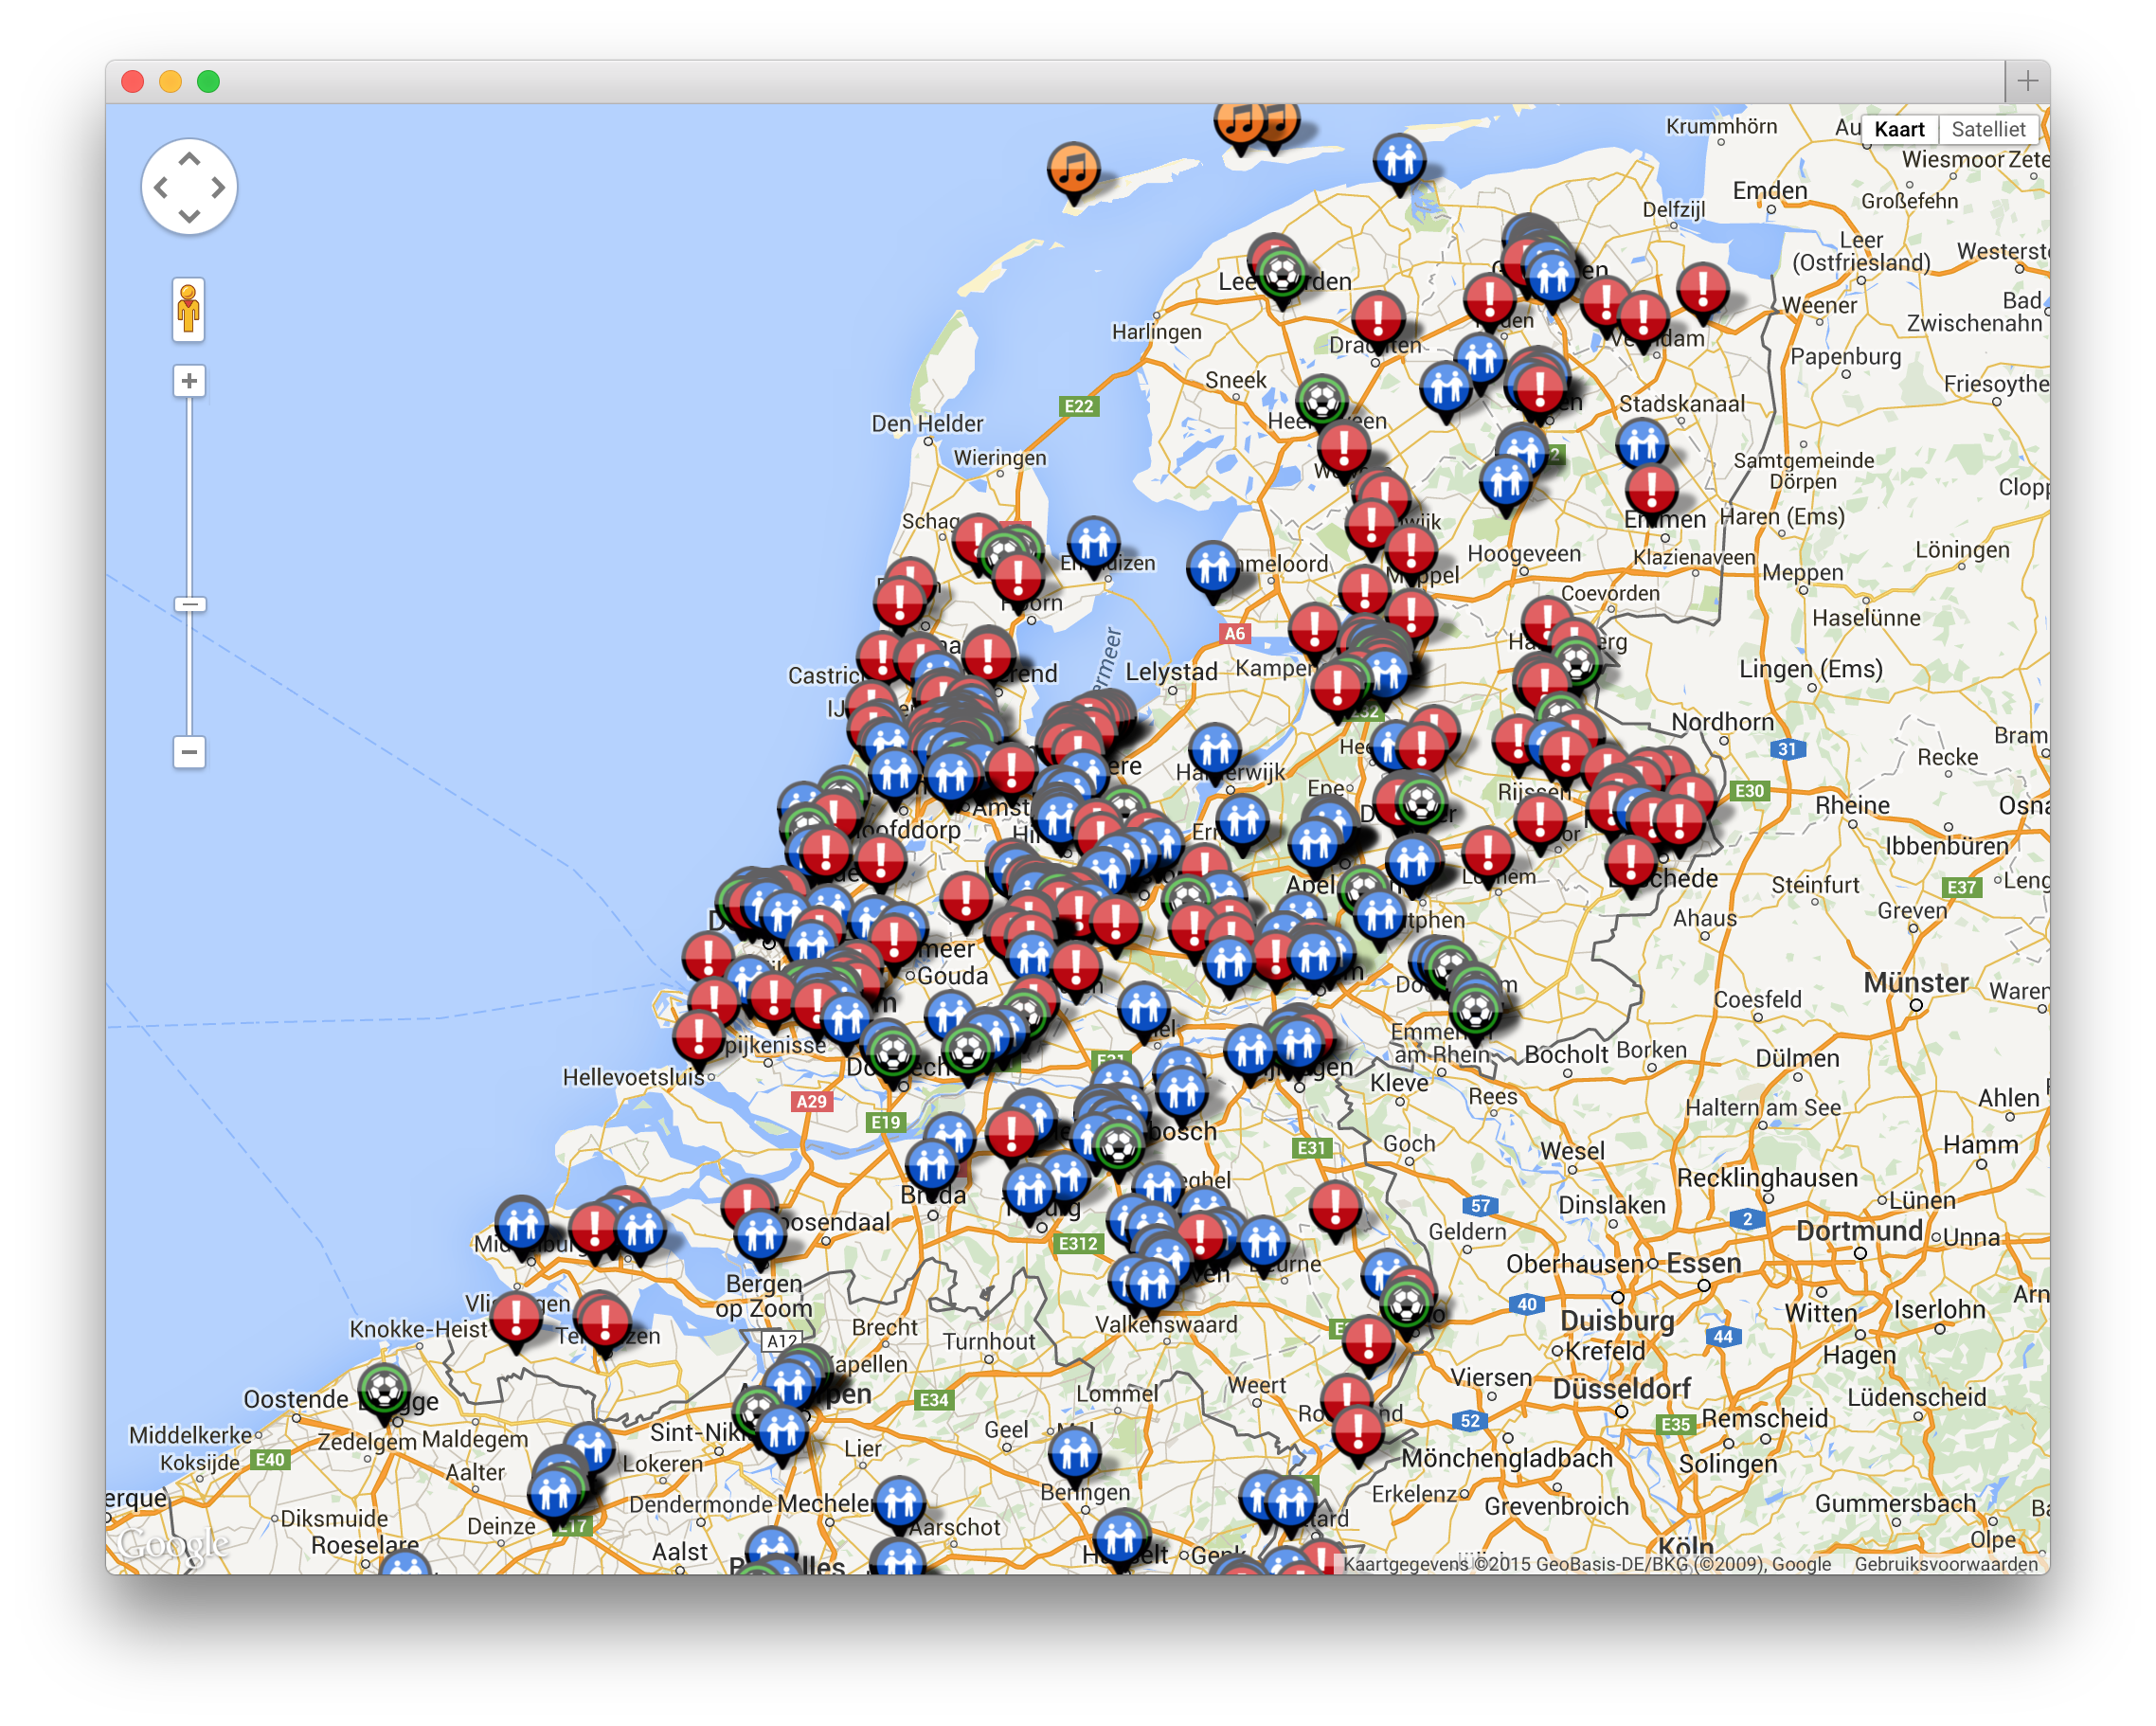
\includegraphics[width=4.5in]{voorkant.png} 
   \label{fig:gui}
\end{figure}
\thispagestyle{empty}
\vfill \noindent Chris Pool\\
S2816539\\
June 14, 2015
\end{titlepage}

%----------------------------------------------------------------------------------------
%	Preface
%----------------------------------------------------------------------------------------
\newpage
\begin{titlepage}
\section*{Preface} % This section will not appear in the table of contents due to the star (\section*)
This thesis is written as part of my Bachelor Information sciences at the University of Groningen that is part of my one year pre-master.  
\vl
I would like to thank my supervisors Malvina Nissim and Johan Bos for helping me during my research. I would also like to thank Rob van der Goot, PhD at the University of Groningen who helped me with creating a Named Entity Classifier.
\vl
Most of the programming is done together with David de Kleer, I would especially like to thank him for the pleasant collaboration.
\vl
\textit{Chris Pool}
\pagestyle{empty}
\end{titlepage}

%----------------------------------------------------------------------------------------
%	TABLE OF CONTENTS & LISTS OF FIGURES AND TABLES
%----------------------------------------------------------------------------------------
\newpage
\setcounter{tocdepth}{3} % Set the depth of the table of contents to show sections and subsections only
\tableofcontents % Print the table of contents

\listoffigures % Print the list of figures

\listoftables % Print the list of tables

\lstlistoflistings
%----------------------------------------------------------------------------------------
%	ABSTRACT
%----------------------------------------------------------------------------------------
\newpage
\section*{Abstract} % This section will not appear in the table of contents due to the star (\section*)
\markboth{Abstract}{Abstract}
With the growing number of people using social media services like Twitter it becomes interesting to use this enormous amount of data as a source of information about things happening at a certain location and time. 
\vl
The goal of my research is to develop a system that uses tweets with geo-information to detect events taking place at a specific location, for example concerts, football matches, fires or traffic jams and recognize the named entities in those events. Events that take place on a larger scale like elections and extreme weather conditions are ignored. This event detection part of my research is done together with David de Kleer, student at the University of Groningen. For the the final part of my research I developed a system that can detect important entities in the events returned by the system.
\vl
The first step is collecting the data. We used the tweets available on the Karora server\footnote{Linux server available for students and staff of the University of Groningen}. This server stores all Dutch tweets and can be easily accessed. We downloaded all tweets with geo-information published in May 2015 to use in developing the system. Tweets from the last two weeks in April 2015 are used to test the system.
\vl
The second step is to create clusters of collected tweets, these clusters are potential events that we call \textit{eventCandidates}. We create these \textit{eventCandidates} by clustering tweets by location and time. To make these \textit{eventCandidates} an algorithm is used called GeoHash, this  algorithm converts latitude and longitude coordinates into a hash, this hash indicates an area where the location is in. The more digits used for this hash, the smaller the area, and thus more accurate. For clustering by time I use the UNIX timestamp, this timestamp is a system that represents time in seconds since 1 January 1970.
\vl
We both annotated the same datasets making it possible to calculate the inter-annotator agreement, the result is a kappa score of 0.79 for our training set en 0.8 for our test set, bot scores indicate a good agreement(\citealt{manning2008introduction}). With the annotated data we trained a Naive Bayes classifier using NLTK. Using the development dataset as training data and the test dataset as test data this resulted in an accuracy of 84\%, with a upperbound of 86\% and baseline of 46\%\footnote{Baseline: Every event candidate is regarded as no event which is the largest category} we see this as a good result.
\vl
With the classified \textit{eventCandidates} using the categories: No event, Meeting, Entertainment, Incident, Sport and Other I tried to detect named entities within those events. The Stanford Named Entity Recognizer was trained using automatically annotated tweets. The results are reasonable, but it shows the difficulty in detecting entities in such short and noisy pieces of text.
\vl
The events, including the named entities, are plotted on a Google map making it easy to check out the events.

%----------------------------------------------------------------------------------------

\newpage % Start the article content on the second page, remove this if you have a longer abstract that goes onto the second page

%----------------------------------------------------------------------------------------
%	INTRODUCTION
%----------------------------------------------------------------------------------------

\section{Introduction}

%waarom
With the growing number of people using social media services like Twitter makes it interesting to use this enormous amount of data as a source of information about things happening at a certain location and time. 
\vl
About 3\% of all tweets contains geo-information\footnote{Based on my own data, see chapter 2 for literature research}. That looks like a small portion but because of the enormous amount of tweets available this gives great insights about the opinion of users at a certain location. This can be used for example to provide news items with more information about the opinion of people. The research of \citeauthor{walther2013geo} was an inspiration for this research. They did a research about event detection using tweets from the New York metropolitan area.
\vl
This event detection part of my research is done together with David de Kleer, student at the University of Groningen. The final part of my research was to develop a system that can detect named entities in the events. 
\vl
This thesis describes a method of finding local events in the Netherlands based on tweets with geo-information and categorizing them into five categories (No-event, Sport, Entertainment, Meeting and Incident). Also a method to find relevant information within those events about the location and people involved is described. 
\vl
My research questions are:
\begin{enumerate}[noitemsep]
\item Is it possible to automatically detect local events in the Twitter stream that take place in the Netherlands based on Tweets with geo-information?
\item if so, is it possible to detect what type of event it is?
\item and is it possible to detect the important entities in these events?
\end{enumerate}

\noindent This thesis is divided in four chapters. The first chapter, related literature, describes the research that has already been done about this subject. The second chapter is the method section where I describe the methods we used for our experiment. In the third chapter I describe our experiment, all code I am referring to can also be found in the GitHub repository\footnote{http://www.github.com/chrispool/thesis}. In the final chapter you can find my conclusion.
%----------------------------------------------------------------------------------------
%	Related literature
%----------------------------------------------------------------------------------------
\newpage
\section{Related literature}
In our research we try to detect events in a large amount of data , in our case tweets. Event detection in newspapers and other media has been addressed in the TDT research program, this program tries to find and follow events in news stories published in newspapers or shown on TV. According to \citet{allan1998topic} events can be defined as \textit{"real-world occurrences that unfold over space and time"} (\citealt{allan1998topic}). 
\vl
Since the launch of Twitter in 2006 the popularity of this micro-blogging service is increasing rapidly. With 302 million users sending about 500 million tweets per day this is a huge source of information (\citealt{statista}). 
In the Netherlands the number of active users was 2.8 million in 2015 according to the research conducted by \citet{newcom}. 
\vl
Unfortunately there are no figures available about the number of tweets with geo-information. Doing a small test on our own data has shown that about 3\% of tweets has geo-information. Figure 1 is a heatmap of tweets with geo-information and shows a lot of tweets in the Netherlands. The Netherlands is one of the countries with the highest twitter accounts to population ratio (\citealt{dawson}).
\begin{figure}[htbp] %  figure placement: here, top, bottom, or page
   \centering
   \includegraphics[width=4in]{MiguelRios_Europe.jpg} 
   \caption{Tweets with geo-information (\citealt{rios})}
   \label{fig:example}
\end{figure}

\noindent Using geo-information from tweets has been done in several works, for example \citet{sakaki2010earthquake} in their paper \textit{Earthquake shakes Twitter users: real-time event detection by social sensors} uses geo-information of tweets to detect earthquakes by analyzing all tweets that contain certain keywords like \textit{earthquake} or \textit{shaking}. In the research by \citet{walther2013geo} they describe the process of detecting events in the Twitter stream, this research was the inspiration for my research and builds on several techniques they discuss. 
\vl
Data clustering is a field where a lot of research is done but according to \citet{birant2007st} most studies focus on discovering clusters from ordinary data (non-spatial and non-temporal data), so they are impractical to use for clustering spatial-temporal data. They see knowledge discovery from spatial-temporal data as very promising (\citealt{birant2007st}). There are five different types of clustering algorithms: Partitional, Hierarchical, Grid-based, Model-based and Density-based (\citealt{han2006data}). Because most algorithms cluster the data using a frozen dataset it is not possible to add values without clustering the data again making it impossible for real-time use. 
\vl
GeoHash is is a system invented by Gustavo Niemeyer\footnote{http://en.wikipedia.org/wiki/Geohash} that converts latitude and longitude coordinates into a \textit{geoHash}. The hash represents an area where in the location is present. The length of the hash indicates the precision, more digits used indicates a smaller area, and thus a higher precision. This grid based algorithm can be used to make clusters of our tweets that works very fast and can also be used in real-time.
\vl
For detecting important entities in the events I want to use Named Entity Recognition. NER is the proces of labeling data with corresponding categories like person, organization or location (\citealt{manning2008introduction}). Current NER tools were designed to process large texts and perform poorly with tweets due to the noisy and short style of tweets, also the limit of 140 characters makes it difficult to recognize entities because the lack of context (\citealt{ner2011} and \citealt{liu2011ner}). A key feature for named entity recognition is the use of capital letters, unfortunately the use of capital letters in tweets if often less reliably and make it hard to recognize entities. According to \citet{ner2011} the Stanford NER, a state of the art classifier, focusses to much on capital letters making it perform poorly on tweets.



%----------------------------------------------------------------------------------------
%	METHOD
%----------------------------------------------------------------------------------------
\newpage
\section{Data en Method}
The goal of my research is to develop a system that can detect events that take place at a specific location, for example concerts, football matches, fires and traffic jams and recognize the named entities in those events. Events that take place on a larger scale like elections and extreme weather conditions are ignored. This chapter describes the methods used in our system and the motivation why we chose these methods.

\subsection{Data collection}
For the experiment tweets are used that have geo-information. Using a simple Grep\footnote{Command-line utility for searching plain-text data sets for lines matching a regular expression } command it was possible to retrieve only tweets with this information from the Linux server \textit{Karora}\footnote{karora.let.rug.nl} that is available for students and staff of the University of Groningen. For our system we retrieved two datasets, one for training and developing our system that we call \textit{devset} and one for testing our final system that we call \textit{testset}
The \textit{devset} consists of Dutch tweets posted in March 2015 that we have downloaded from \textit{Karora}. In total there where 566,549 tweets with geo-information. That is about 3\% of the total number of tweets published in that month. The \textit{testset} consists of 165,848 tweets published in the second half of April 2015. The tweets are stored in a tab separated text file with the fields tweet, latitude, longitude, username and timestamp


\subsection{Pipeline}
\begin{figure}[htbp] %  figure placement: here, top, bottom, or page
   \centering
   \includegraphics[width=4in]{pipeline.png} 
   \caption{Pipeline}
   \label{fig:example}
\end{figure}
\noindent The process is to first cluster the tweets by location and time and  to determine if the clusters are events or not and if so, which type of event it is. The final step is to detect the interesting entities in the events. In this section you can find a description of the used methods. The implementation can be found in the next chapter.
\newpage
\subsubsection{Clustering}
The first task is to cluster the tweets by location and time. There are several approaches in location clustering that can be used as discussed in the previous chapter. We wanted to use a clustering algorithm that potentially could work in real-time so it was necessary to look for an approach that was quick and accurate. GeoHash is is a system invented by Gustavo Niemeyer\footnote{http://en.wikipedia.org/wiki/Geohash} that converts latitude and longitude coordinates into a \textit{geoHash}. The hash represents an area where in the location is present. The length of the hash indicates the precision, more digits used indicates a smaller area, and thus a higher precision. If two locations share the same prefix it indicates (not always\footnote{Some neighboring geoHashes start with a different character as can be seen in figure 1 }) that the locations are nearby. 
\begin{figure}[htbp] %  figure placement: here, top, bottom, or page
   \centering
   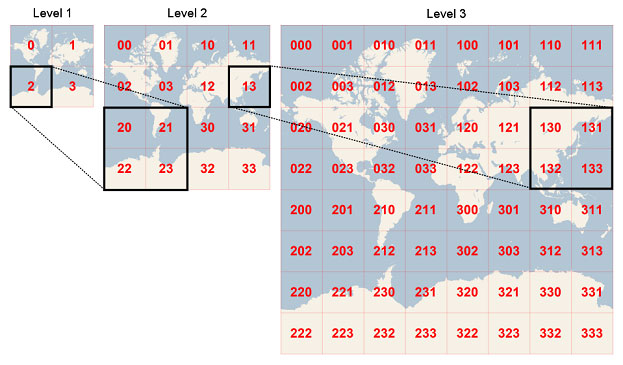
\includegraphics[width=4.5in]{geohash.jpg} 
   \caption{Geohash}
   \label{fig:geohash}
\end{figure}
\vl
 Figure 1 illustrates how geoHash works. The first digit indicates which halve of the earth the area is on. The second digit divides that area in four areas and that continues resulting in table 1 that shows the different lengths of the \textit{geoHash} and the accuracy of that length. Because the dimensions of the area are different at each latitude the values represent the worst-case scenario at the equator.

\begin{table}[h]
\caption[Geohash Precision]{Geohash Precision}
\begin{tabular}{|c|c|}
\hline
GeoHash length & Area width x height   \\ \hline
1              & 5,009.4km x 4,992.6km \\ \hline
2              & 1,252.3km x 624.1km   \\ \hline
3              & 156.5km x 156km       \\ \hline
4              & 39.1km x 19.5km       \\ \hline
5              & 4.9km x 4.9km         \\ \hline
6              & 1.2km x 609.4m        \\ \hline
7              & 152.9m x 152.4m       \\ \hline
8              & 38.2m x 19m           \\ \hline
9              & 4.8m x 4.8m           \\ \hline
10             & 1.2m x 59.5cm         \\ \hline
11             & 14.9cm x 14.9cm       \\ \hline
12             & 3.7cm x 1.9cm         \\ \hline
\end{tabular}
\end{table}
\newpage
\noindent There are several implementations of this algorithm in Python. We used the GeoHash library written in 2009 by Hiroaki Kawai\footnote{https://github.com/hkwi/python-geohash} because of the good documentation and excellent features. The function to calculate the \textit{geoHash} of a location requires the desired accuracy, latitude and longitude of that location and returns the \textit{geoHash} for that location as can be seen in code example 1. \vl

\begin{lstlisting}[language=Python, caption=Example of geoHash encoding]
lon = 52.348
lat = 6.2342
accuracy = 7

hash = geohash.encode(lon,lat,accuracy)
>>> print(hash)
u1k3y1c
\end{lstlisting}
This library also provides functions to calculate the neighboring geoHashes and this is useful because in a grid clustering approach border cases can occur.  We use this functionality to merge our neighboring \textit{eventCandidates} as described in 4.3 Creating eventCandidates. \vl
For clustering timestamps the UNIX timestamp can be used. This is a system to represent time using the number of seconds since 1 January 1970. Python has built-in functions to deal with UNIX timestamps. The tweets are sorted on timestamp making it easy to make clusters of time series. The implementation of these functions can be found in chapter 3.3 Event Detection.


\subsubsection{Classification}
After forming the potential events (\textit{eventCandidates}) the Event Candidates have to be classified using the categories: 

\begin{itemize}[noitemsep]
\item No Event
\item Meeting
\item Entertainment
\item Incident
\item Sport
\item Other
\end{itemize}

\noindent We decided for these categories because after looking at the data these made the most sense. The Meeting category, which is to largest in both datasets, could be divided further. For example political meetings or rallies ,congresses and book presentations are part of this category but for our goal, to plot them on a Google map we did not want to use too many categories. It is possible to train the classifier with other categories but requires a new annotation.
\vl
In our experiment we have chosen to use the MaxEntClassifier, NaiveBayes and a SVM classifier. Using NLTK it was easy to train the classifiers. Each classifier requires the same format of train data making it easy to compare the results of the different classifiers. In chapter 4 you can find a more detailed description about training the classifiers.

\subsubsection{Named Entity Recognition}
For finding the important persons, organizations and locations I want to use Named Entity Recognition(NER). NER is the proces of labeling data with corresponding categories like person, organization or location. For example:

\begin {quote}
Na 14 minuten is het raak! 1-0 voor \textbf{Woudrichem(Organization)}. Doelpunt \textbf{Roy van Sonsbeek(Person)}
\end{quote}

\noindent As discussed in chapter 2 the standard NER classifiers perform poorly with tweets, therefore I decided to train my own classifier to detect named entities. With help from Rob van der Goot, PhD student at the University of Groningen I created an automatically annotated dataset that I want to use to train a classifier. I do this by using lists of Dutch words for each category (Location, Person, Organization and Miscellaneous) and label those words in downloaded tweets creating a sliver standard. 
\vl
The purpose of training a classifier and not using a word list for named entity detection is that the word lists contains well known entities like \textit{Ajax} and \textit{Feyenoord} but not the name of the local football club and those frequent occurring local entities I want to recognize. The detailed explanation of training the classifier can be found in chapter 4. 

\subsection{Evaluation}
For evaluating event detection we annotated both datasets by giving all \textit{eventCandidates} a label. We created a gold standard by removing all \textit{eventCandidates} we did not agree on. With this gold standard we can calculate the precision, recall and F-score of our system for each category and overal accuracy (\citealt{manning2008introduction}). For the named entity recognition we can also calculate the precision, recall and f-score for each category.  For the event detection we use the largest category as baseline which is the no-event category(40\%) and for upper-bound we use the annotation accuracy (86\%).

%----------------------------------------------------------------------------------------
%	Experiment and Evaluation
%----------------------------------------------------------------------------------------
\newpage
\section{Implementation and results}
For our experiment I worked together with David de Kleer in collecting the data and building the Python modules. The goal was to build a system that can detect events that take place at a specific location, for example concerts, football matches, fires and traffic jams and recognize the named entities in those events.  Events that take place on a larger scale like elections and extreme weather conditions are ignored. The input for this system are tweets that have coordinates that we cluster by location and time. These clusters of tweets are potential events (\textit{eventCandidates}) that the system classifies using the following categories: \newline

\begin{itemize}[noitemsep] % [noitemsep] removes whitespace between the items for a compact look
\item \textbf{Other (OTH)} All events that are other then the following categories 
\item \textbf{Meeting (MEE)} All events that are meetings or conferences 
\item \textbf{Entertainment (ENT)} All events that have to do with concerts, movies or theater
\item \textbf{No Event (NOE)} No Event
\item \textbf{Incident (INC)} Events that have to do with an incident
\item \textbf{Sport (SPO)} All events that have to do with sport 
\end{itemize}


\subsection{System architecture}
Python was used as the programming language for this system because of the excellent tools available to build a machine learning system. NLTK and Scikit learn are used for classifying \textit{eventCandidates}. GitHub\footnote{http://www.gitHub.com/chrispool/thesis} was used as file repository. The system consists of five different modules each containing multiple scripts. In this section the main properties of the modules are described. In the following sections the modules are explained in detail.

\begin{description}

\item[EventCandidates] 
The module that generates the \textit{eventCandidates} by clustering the tweets by \textit{geoHash} and timestamp and saves the result as a JSON file.  

\item[Annotator] 
The module that makes it possible for multiple judges to annotate the data created with the EventCandidates module and calculates the inter-annotator agreement. 

\item[ClassifierCreator] 
The module that creates/trains the classifier(s) using the annotated \textit{eventCandidates.}

\item[EventDetective] 
The module that uses the trained classifier to classify eventCandidates and generate markers for the Google map.

\item[NER]
The module that uses the NER classifier that is explained in the Named Entity Recognition section of this chapter.  

\end{description}

\newpage


\subsection{Creating Event Candidates}
For clustering the tweets and preparing them for annotation and classification we use the EventCandidates module. This module processes all tweets from a given dataset and generates the \textit{eventCandidates} using four scripts. TweetPreprocessor.py, ClusterCreator.py, ClusterMerger.py and EventCandidates.py

\paragraph{TweetPreprocessor.py}reads the text file with tweets and tokenizes the tweets and removes the frequent occurring words from the tokens, convert the time string to a Unix timestamp and converts the latitude en longitude into a geoHash. The output of this script is a list of dictionaries where each dictionary is a tweet with the structure as found in code example 2.

\begin{lstlisting}[language=Python, caption=Tweet dictionary]
{'text': '@MrFrankLegs Daar gaan we. Een vicieuze cirkel ??', 
'lat': 52.964285, 
'geoHash': 'u1kjqcc', 
'localTime': '2015-04-24 10:54:16', 
'user': 'sandersierdsma', 
'tokens': ['@mrfranklegs', 'gaan', 'vicieuze', 'cirkel'], 
'lon': 5.923195, 
'unixTime': 1429865656}
\end{lstlisting}
\paragraph{ClusterCreator.py} iterates over all tweet dictionaries and adds the tweet dictionary to a list in the new two-dimensional dictionary as seen in code example 3. With as first key the geoHash and the second key the Unix timestamp of the last added tweet. 
\begin{lstlisting}[language=Python, caption=Result dictionary]
clusters['u15y07t']['1429604082'] = [...list of tweet dictionaries...]
\end{lstlisting}
With this two-dimensional dictionary we can check for each tweet if we can add it to an existing \textit{eventCandidate} or that we have to create a new \textit{eventCandidate}. 

We do this by iterating over all tweet and try to append the tweet to the dictionary described in code example 3. We first look if the geoHash of the tweet is present in the dictionary, if not a new entry is added with the geoHash as key. If the geoHash is present we look if there is a timestamp as key that is within 60 minutes of the tweet, if so we append it to this cluster, if not we create a new cluster(\textit{eventCandidate})

\paragraph{ClusterMerger.py} checks if there are clusters that overlap in time and subject and are neighboring areas. For example the situation in figure 2, the tweets (red dots) are all about the same event and published in the same period but they are in two different areas.  

\begin{figure}[htbp] %  figure placement: here, top, bottom, or page
   \centering
   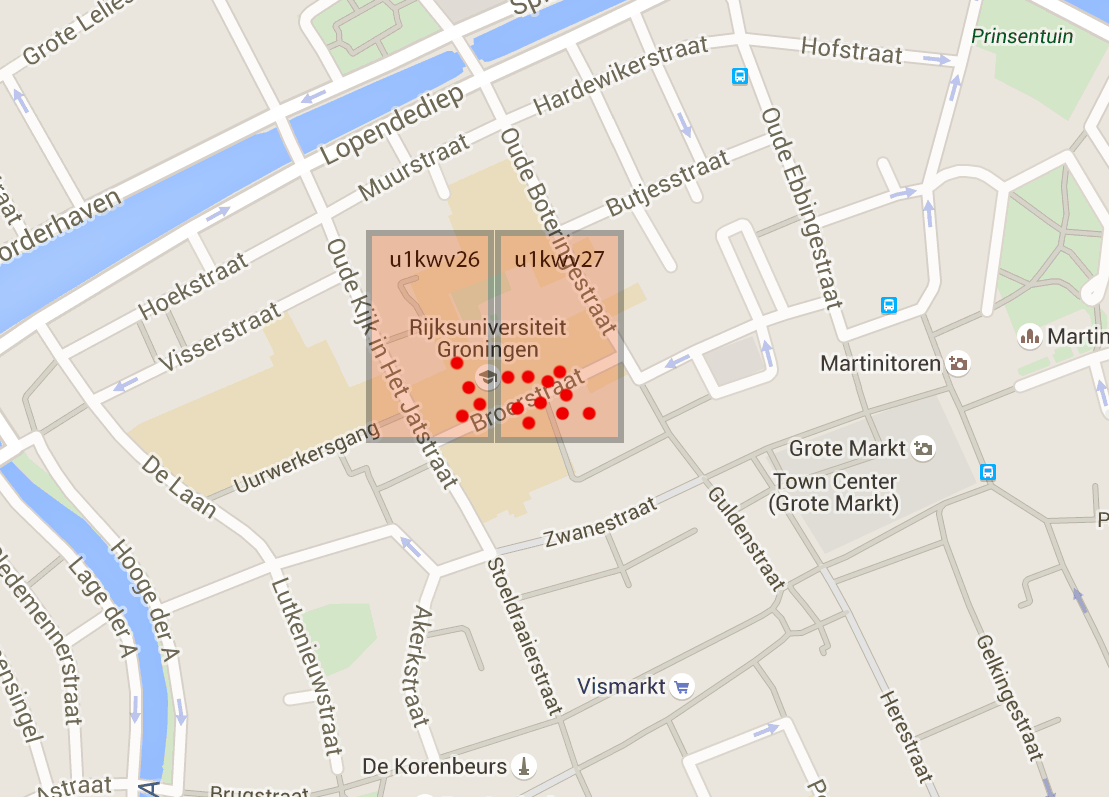
\includegraphics[width=3in]{bordercase.png} 
   \caption{Geohash border case}
   \label{Geohash border case}
\end{figure}
The ClusterMerger.py script tries to merge situations as described.  We do this by iterating over the \textit{eventCandidates} and calculate all neighbors of the current \textit{eventCandidate}. We then iterate over all neighboring areas and if an \textit{eventCandidate} is found we calculate the word overlap (code example 4) to see if the \textit{eventCandidates} refer to the same event. If that is the case we merge the \textit{eventCandidates} and continue the loop until all neighboring areas are checked.
\vl
During the development of our system we discussed the number of iterations. If you iterate only once you will merge only the neighbors next to you. You can do this more than once to merge the neighbors of the neighbors etc. We chose to use only one iteration because we want local events that take place at a small area.
\vl
We calculate the word overlap to see if the two \textit{eventCandidates} refer to the same event.  The function \textit{calculteWordOverlap}(code example 5) does that by looking at the 10 most common word in both clusters. For each word that overlaps a score of one time the tf-idf\footnote{term frequency - inverse document frequency, used to reflect how important a word is in a corpus} value is awarded. If a hashtag or username overlaps the score is tf-idf * 2. If the total score exceeds the threshold the function returns true. 

\begin{lstlisting}[language=Python, caption=Calculate word overlap]
def _calculateWordOverlap(self,clusterA, clusterB):      
    wordsClusterA = self._getImportantWords(10, clusterA)
    wordsClusterB = self._getImportantWords(10, clusterB)
    result = {}
    
    #intersect the two lists and adding the scores
    for wordA, scoreA in wordsClusterA:
        for wordB, scoreB in wordsClusterB:
            if wordA == wordB:
                result[wordA] = scoreA + scoreB
                if wordA[0] == '#':
                    result[wordA] *= 2
                if wordA[0] == '@':
                    result[wordA] *= 2

    if sum(result.values()) > self.THRESHOLD:
        return True
    else:
        return False
\end{lstlisting}


\paragraph{EventCandidates.py} is the wrapper class for this module. This script generates all \textit{eventCandidates} using the scripts described above. This function requires two parameters. The first is the name of the text file with the unprocessed tweets. The second is the desired name of the dataset. This script saves a JSON file with all \textit{eventCandidates}.

\subsection{Annotation}
This module consists of two scripts: Annotator.py and AnnotationEvaluation.py.

\paragraph{Annotator.py}  is an interactive program to annotate the created \textit{eventCandidates} using the Event candidates module. The program shows all tweets in the \textit{eventCandidate} and prompts you to assign a category to them and saves the result in a JSON file. We used Annotator.py for two datasets: \textit{devset}(1250 \textit{eventCandidates}) and \textit{testset}(500 \textit{eventCandidates}). We annotated the \textit{devtest} in the beginning of our research and the \textit{testset} dataset in the final period of our research. The annotation is done with two annotators making it possible to calculate the inter-annotator agreement.

\paragraph{AnnotationEvaluation.py} is used to calculate the inter-annotator agreement. This is a statistic to determine the quality of annotation and also shows how difficult the task is. We use these statistics also to define our upper-bound. In table 2 the results of the annotation can be found. A kappa score of 0.79 and 0.8 is regarded as good (\citealt{manning2008introduction}).

\begin{table}[h]
 \centering
\caption[Annotation result]{Annotation result }
\begin{tabular}{|c|c|c|}
\hline
              & Kappa score & Accuracy \\ \hline
{\it devset}  & 0.79  & 87\%     \\ \hline
{\it testset} & 0.80  & 86\%     \\ \hline
\end{tabular}
\end{table}

\noindent The confusion matrixes shows the confusion between both judges. Some categories have a higher accuracy because it is easier to detect. For example a lot of \textit{eventCandidates} annotated as a incident have words like \textit{112} or \textit{brandweer} in them where as in the Meeting category it was sometimes unclear if it was an event. 
\begin{table}[h]
 \centering
\caption[Confusion matrix testset annotation]{Confusion matrix development dataset annotation }
\begin{tabular}{lcccccc}
 & \multicolumn{1}{l}{\textbf{OTH}} & \multicolumn{1}{l}{\textbf{MEE}} & \multicolumn{1}{l}{\textbf{ENT}} & \multicolumn{1}{l}{\textbf{NOE}} & \multicolumn{1}{l}{\textbf{INC}} & \multicolumn{1}{l}{\textbf{SPO}} \\ \cline{2-7} 
\multicolumn{1}{l|}{\textbf{OTH}} & \multicolumn{1}{c|}{\textless1\textgreater} & \multicolumn{1}{c|}{.} & \multicolumn{1}{c|}{.} & \multicolumn{1}{c|}{2} & \multicolumn{1}{c|}{1} & \multicolumn{1}{c|}{1} \\ \cline{2-7} 
\multicolumn{1}{l|}{\textbf{MEE}} & \multicolumn{1}{c|}{21} & \multicolumn{1}{c|}{\textless207\textgreater} & \multicolumn{1}{c|}{7} & \multicolumn{1}{c|}{25} & \multicolumn{1}{c|}{.} & \multicolumn{1}{c|}{2} \\ \cline{2-7} 
\multicolumn{1}{l|}{\textbf{ENT}} & \multicolumn{1}{c|}{3} & \multicolumn{1}{c|}{.} & \multicolumn{1}{c|}{\textless20\textgreater} & \multicolumn{1}{c|}{5} & \multicolumn{1}{c|}{.} & \multicolumn{1}{c|}{.} \\ \cline{2-7} 
\multicolumn{1}{l|}{\textbf{NOE}} & \multicolumn{1}{c|}{14} & \multicolumn{1}{c|}{27} & \multicolumn{1}{c|}{18} & \multicolumn{1}{c|}{\textless619\textgreater} & \multicolumn{1}{c|}{9} & \multicolumn{1}{c|}{9} \\ \cline{2-7} 
\multicolumn{1}{l|}{\textbf{INC}} & \multicolumn{1}{c|}{1} & \multicolumn{1}{c|}{2} & \multicolumn{1}{c|}{.} & \multicolumn{1}{c|}{12} & \multicolumn{1}{c|}{\textless178\textgreater} & \multicolumn{1}{c|}{.} \\ \cline{2-7} 
\multicolumn{1}{l|}{\textbf{SPO}} & \multicolumn{1}{c|}{1} & \multicolumn{1}{c|}{.} & \multicolumn{1}{c|}{.} & \multicolumn{1}{c|}{5} & \multicolumn{1}{c|}{.} & \multicolumn{1}{c|}{\textless60\textgreater} \\ \cline{2-7} 
\end{tabular}
\end{table}

\begin{table}[h]
 \centering
\caption[Confusion matrix devset annotation]{Confusion matrix test dataset annotation }
\begin{tabular}{lcccccc}
                                  & \multicolumn{1}{l}{\textbf{OTH}}            & \multicolumn{1}{l}{\textbf{MEE}}              & \multicolumn{1}{l}{\textbf{ENT}}            & \multicolumn{1}{l}{\textbf{NOE}}              & \multicolumn{1}{l}{\textbf{INC}}             & \multicolumn{1}{l}{\textbf{SPO}}    \\ \cline{2-7} 
\multicolumn{1}{l|}{\textbf{OTH}} & \multicolumn{1}{c|}{\textless.\textgreater} & \multicolumn{1}{c|}{.}                        & \multicolumn{1}{c|}{.}                      & \multicolumn{1}{c|}{.}                        & \multicolumn{1}{c|}{1}                       & \multicolumn{1}{c|}{.}              \\ \cline{2-7} 
\multicolumn{1}{l|}{\textbf{MEE}} & \multicolumn{1}{c|}{4}                      & \multicolumn{1}{c|}{\textless110\textgreater} & \multicolumn{1}{c|}{13}                     & \multicolumn{1}{c|}{9}                        & \multicolumn{1}{c|}{.}                       & \multicolumn{1}{c|}{3}              \\ \cline{2-7} 
\multicolumn{1}{l|}{\textbf{ENT}} & \multicolumn{1}{c|}{.}                      & \multicolumn{1}{c|}{.}                        & \multicolumn{1}{c|}{\textless8\textgreater} & \multicolumn{1}{c|}{2}                        & \multicolumn{1}{c|}{.}                       & \multicolumn{1}{c|}{.}              \\ \cline{2-7} 
\multicolumn{1}{l|}{\textbf{NOE}} & \multicolumn{1}{c|}{3}                      & \multicolumn{1}{c|}{19}                       & \multicolumn{1}{c|}{4}                      & \multicolumn{1}{c|}{\textless199\textgreater} & \multicolumn{1}{c|}{4}                       & \multicolumn{1}{c|}{2}              \\ \cline{2-7} 
\multicolumn{1}{l|}{\textbf{INC}} & \multicolumn{1}{c|}{1}                      & \multicolumn{1}{c|}{.}                        & \multicolumn{1}{c|}{.}                      & \multicolumn{1}{c|}{.}                        & \multicolumn{1}{c|}{\textless78\textgreater} & \multicolumn{1}{c|}{.}              \\ \cline{2-7} 
\multicolumn{1}{l|}{\textbf{SPO}} & \multicolumn{1}{c|}{.}                      & \multicolumn{1}{c|}{1}                        & \multicolumn{1}{c|}{2}                      & \multicolumn{1}{c|}{2}                        & \multicolumn{1}{c|}{.}                       & \multicolumn{1}{c|}{\textless8\textgreater} \\ \cline{2-7} 
\end{tabular}

\end{table}


\newpage
\noindent We used the \textit{eventCandidates} we agreed on to create our gold standard. Resulting in 1085 \textit{eventCandidates} in the \textit{devset} and 403 \textit{eventCandidates} in the \textit{testset}.

\begin{figure}[htbp] %  figure placement: here, top, bottom, or page
   \centering
   \includegraphics[width=4in]{annotatieverdeling.png} 
   \caption{Division dataset}
   \label{fig:example}
\end{figure} 
\noindent Figure 5 shows the percentage of the corresponding dataset.

\subsection{Training classifiers}
The ClassifierCreator module has two scripts: classifierCreator.py and featureSelector.py. With the annotation and the \textit{eventCandidates} ready we started with training the classifiers. The module can be used in normal mode and in test mode. The first mode lets you select one dataset and the script divides the dataset in a train and test set (80\%/20\%). In test mode you can select two different datasets, one for training and the other for testing. The test mode was used for calculating the final statistics about our classifier.
\vl
Using the annotation and the \textit{eventCandidates} we start by preparing the training data. We have chosen to use two classifiers, one for classifying using words as features (\textit{categoryClassifier}). And a second classifier using metadata as features (\textit{eventClassifier}). The output of the \textit{categoryClassifer} is used as a feature in the eventClassifier.
\vl
We created featureSelector.py as a helper function that generates the features in the format required by NLTK. We designed this in a very modular way so we could experiment with using different features and combinations of features. 
\vl
This function, as seen in code example 5, requires a list of the desired features and returns the features in a format suitable for training the classifier for a given cluster(\textit{eventCandidate}).\vl
The \textit{categoryClassifier} uses the N most frequent words as features. In order to calculate this feature the system needs to know all used words in the \textit{eventCandidates}, this is done while initializing the features module.

\begin{lstlisting}[language=Python, caption=Selecting features]
def getFeatures(self, candidate, features):
        returnFeatures = {}
        for feature in features:
            if feature in self.featureTypes:
                method = getattr(self, "_" + feature)
                if feature == 'wordFeatures':
                    wordFeatures = method(candidate)
                    #add word features to dictionary to be able to combine features
                    for key in wordFeatures:
                        returnFeatures[key] = wordFeatures[key]
                else:
                    returnFeatures[feature] = method(candidate)
            else:
                print("The feature", feature, "is not available.")

        return returnFeatures
\end{lstlisting}

\noindent With the features in the correct format we can train the classifiers using NLTK, that we also use to calculate the performance of the classifier which can be found in the result section. 
\vl
\begin{lstlisting}[language=Python, caption=Selecting features]
self.classifierBFeatures =  ['category', 'location','wordOverlapSimple','wordOverlapUser']
for candidate, label in self.testData:
            featuresB = self.featureSelector.getFeatures(candidate, self.classifierBFeatures)   
            self.featureKeys = featuresB.keys()
            self.testB.append((featuresB, label)) 
            
for candidate, label in self.trainData:
    featuresB = self.featureSelector.getFeatures(candidate, self.classifierBFeatures)
    self.featureKeys = featuresB.keys()
    self.trainB.append((featuresB, label))

self.classifierB = nltk.NaiveBayesClassifier.train(self.trainB)
\end{lstlisting}




\subsubsection{Feature selection}
The \textit{categoryClassifier} uses the most frequent words as features. The \textit{eventClassifier} uses the output of the first classifier as one of the features. This feature is by far the most valuable for the system. In table 4 the performance of the different features used individual can be found using the \textit{testset}. In appendix 1 the complete results can be found.


\begin{table}[h]
 \centering
\caption[Effect of features]{Effect of features  on testset }
\begin{tabular}{|l|l|}
\hline
                          & Accuracy \\ \hline
All features              & 0.84     \\ \hline
Category                  & 0.81     \\ \hline
Location                  & 0.51     \\ \hline
WordOverlapSimple         & 0.63     \\ \hline
WordOverlapUser           & 0.6      \\ \hline
WordOverlapUser, Category & 0.82     \\ \hline
\end{tabular}

\end{table}

\begin{description}

\item[Category]
The result of the classifier that uses the most frequent words as features. 

\item[Location]
The first 5 characters in the geoHash are used as a feature. It will be easier to detect events on locations were events often take place.

\item[wordOverlapSimple]
This feature is a numeric value that represents how many tweets consist of the same words. The score is calculated by counting the occurrences of each type and dividing it by the number of tweets. Hashtags get a bonus score.

\item[WordOverlapUser]
This feature calculates the overlap of types among users. The score is the highest when all users use the same words. The result is the log of the score and rounded to 0.5.


\end{description}

\subsubsection{Results event detection}
We are very satisfied with the results of our classifier(s). With an accuracy of 84\% it is only a few procent less  than our upper-bound of 87\% and  a lot better then our baseline of 40\%. Naive Bayes was the best performing classifier but the differences where not that big. The table with the precision and recall of each category using Naive Bayes can be found in appendix 1 and the confusion matrixes for all classifiers can be found in appendix 2.

\begin{table}[h]
 \centering
\caption[Results using all features]{Results using all features }
\begin{tabular}{l|l|l|l|l|l|l|l|l|l|}
\cline{2-10}
                          & \multicolumn{3}{c|}{Naive Bayes}                                         & \multicolumn{3}{c|}{Maximum Entropy}                                     & \multicolumn{3}{c|}{SVM}             \\ \cline{2-10} 
                          & \multicolumn{3}{c|}{Accuracy = 84\%}                                     & \multicolumn{3}{c|}{Accuracy = 83\%}                                     & \multicolumn{3}{c|}{Accuracy = 81\%} \\ \cline{2-10} 
                          & \multicolumn{1}{c|}{P} & \multicolumn{1}{c|}{R} & \multicolumn{1}{c|}{F} & \multicolumn{1}{c|}{P} & \multicolumn{1}{c|}{R} & \multicolumn{1}{c|}{F} & P          & R          & F          \\ \hline
\multicolumn{1}{|l|}{NOE} & 0.85                   & 0.90                   & 0.88                   & 0.83                   & 0.93                   & 0.88                   & 0.85       & 0.83       & 0.84       \\ \hline
\multicolumn{1}{|l|}{SPO} & 0.77                   & 0.49                   & 0.60                   & 0.77                   & 0.49                   & 0.60                   & 0.77       & 0.49       & 0.60       \\ \hline
\multicolumn{1}{|l|}{ENT} & 0.00                   & 0.00                   & 0.00                   & 0.00                   & 0.00                   & 0.00                   & 0.00       & 0.00       & 0.00       \\ \hline
\multicolumn{1}{|l|}{MEE} & 0.76                   & 0.79                   & 0.77                   & 0.79                   & 0.74                   & 0.76                   & 0.65       & 0.81       & 0.72       \\ \hline
\multicolumn{1}{|l|}{INC} & 0.97                   & 0.97                   & 0.97                   & 0.94                   & 0.94                   & 0.94                   & 1.00       & 0.97       & 0.99       \\ \hline
\multicolumn{1}{|l|}{OTH} & 0.00                   & 0.00                   & 0.00                   & 0.00                   & 0.00                   & 0.00                   & 0.00       & 0.00       & 0.00       \\ \hline
\end{tabular}

\end{table}

\noindent To compare our research with other researches we also calculated our f-score for all categories except no-event because most researches do binary event-detection (event/ no-event). If we compare our f-score of 88\% with the research of \citeauthor{walther2013geo} (f-score of 86\%) we can see our classifier performs slightly better. A reason could be is that we also use automatically generated tweets of emergency calls that are easy to recognize for our classifier.


\subsection{Event Detective}
This module uses the trained classifiers to generate an interactive map and adds the results of the Named Entity Recognition classifier described in the next section. \vl
To create an interactive map we have chosen to use the Google map API because of the good documentation and excellent features. We generate a javascript file with all information about the markers we want to plot on the map. 

\begin{figure}[htbp] %  figure placement: here, top, bottom, or page
   \centering
   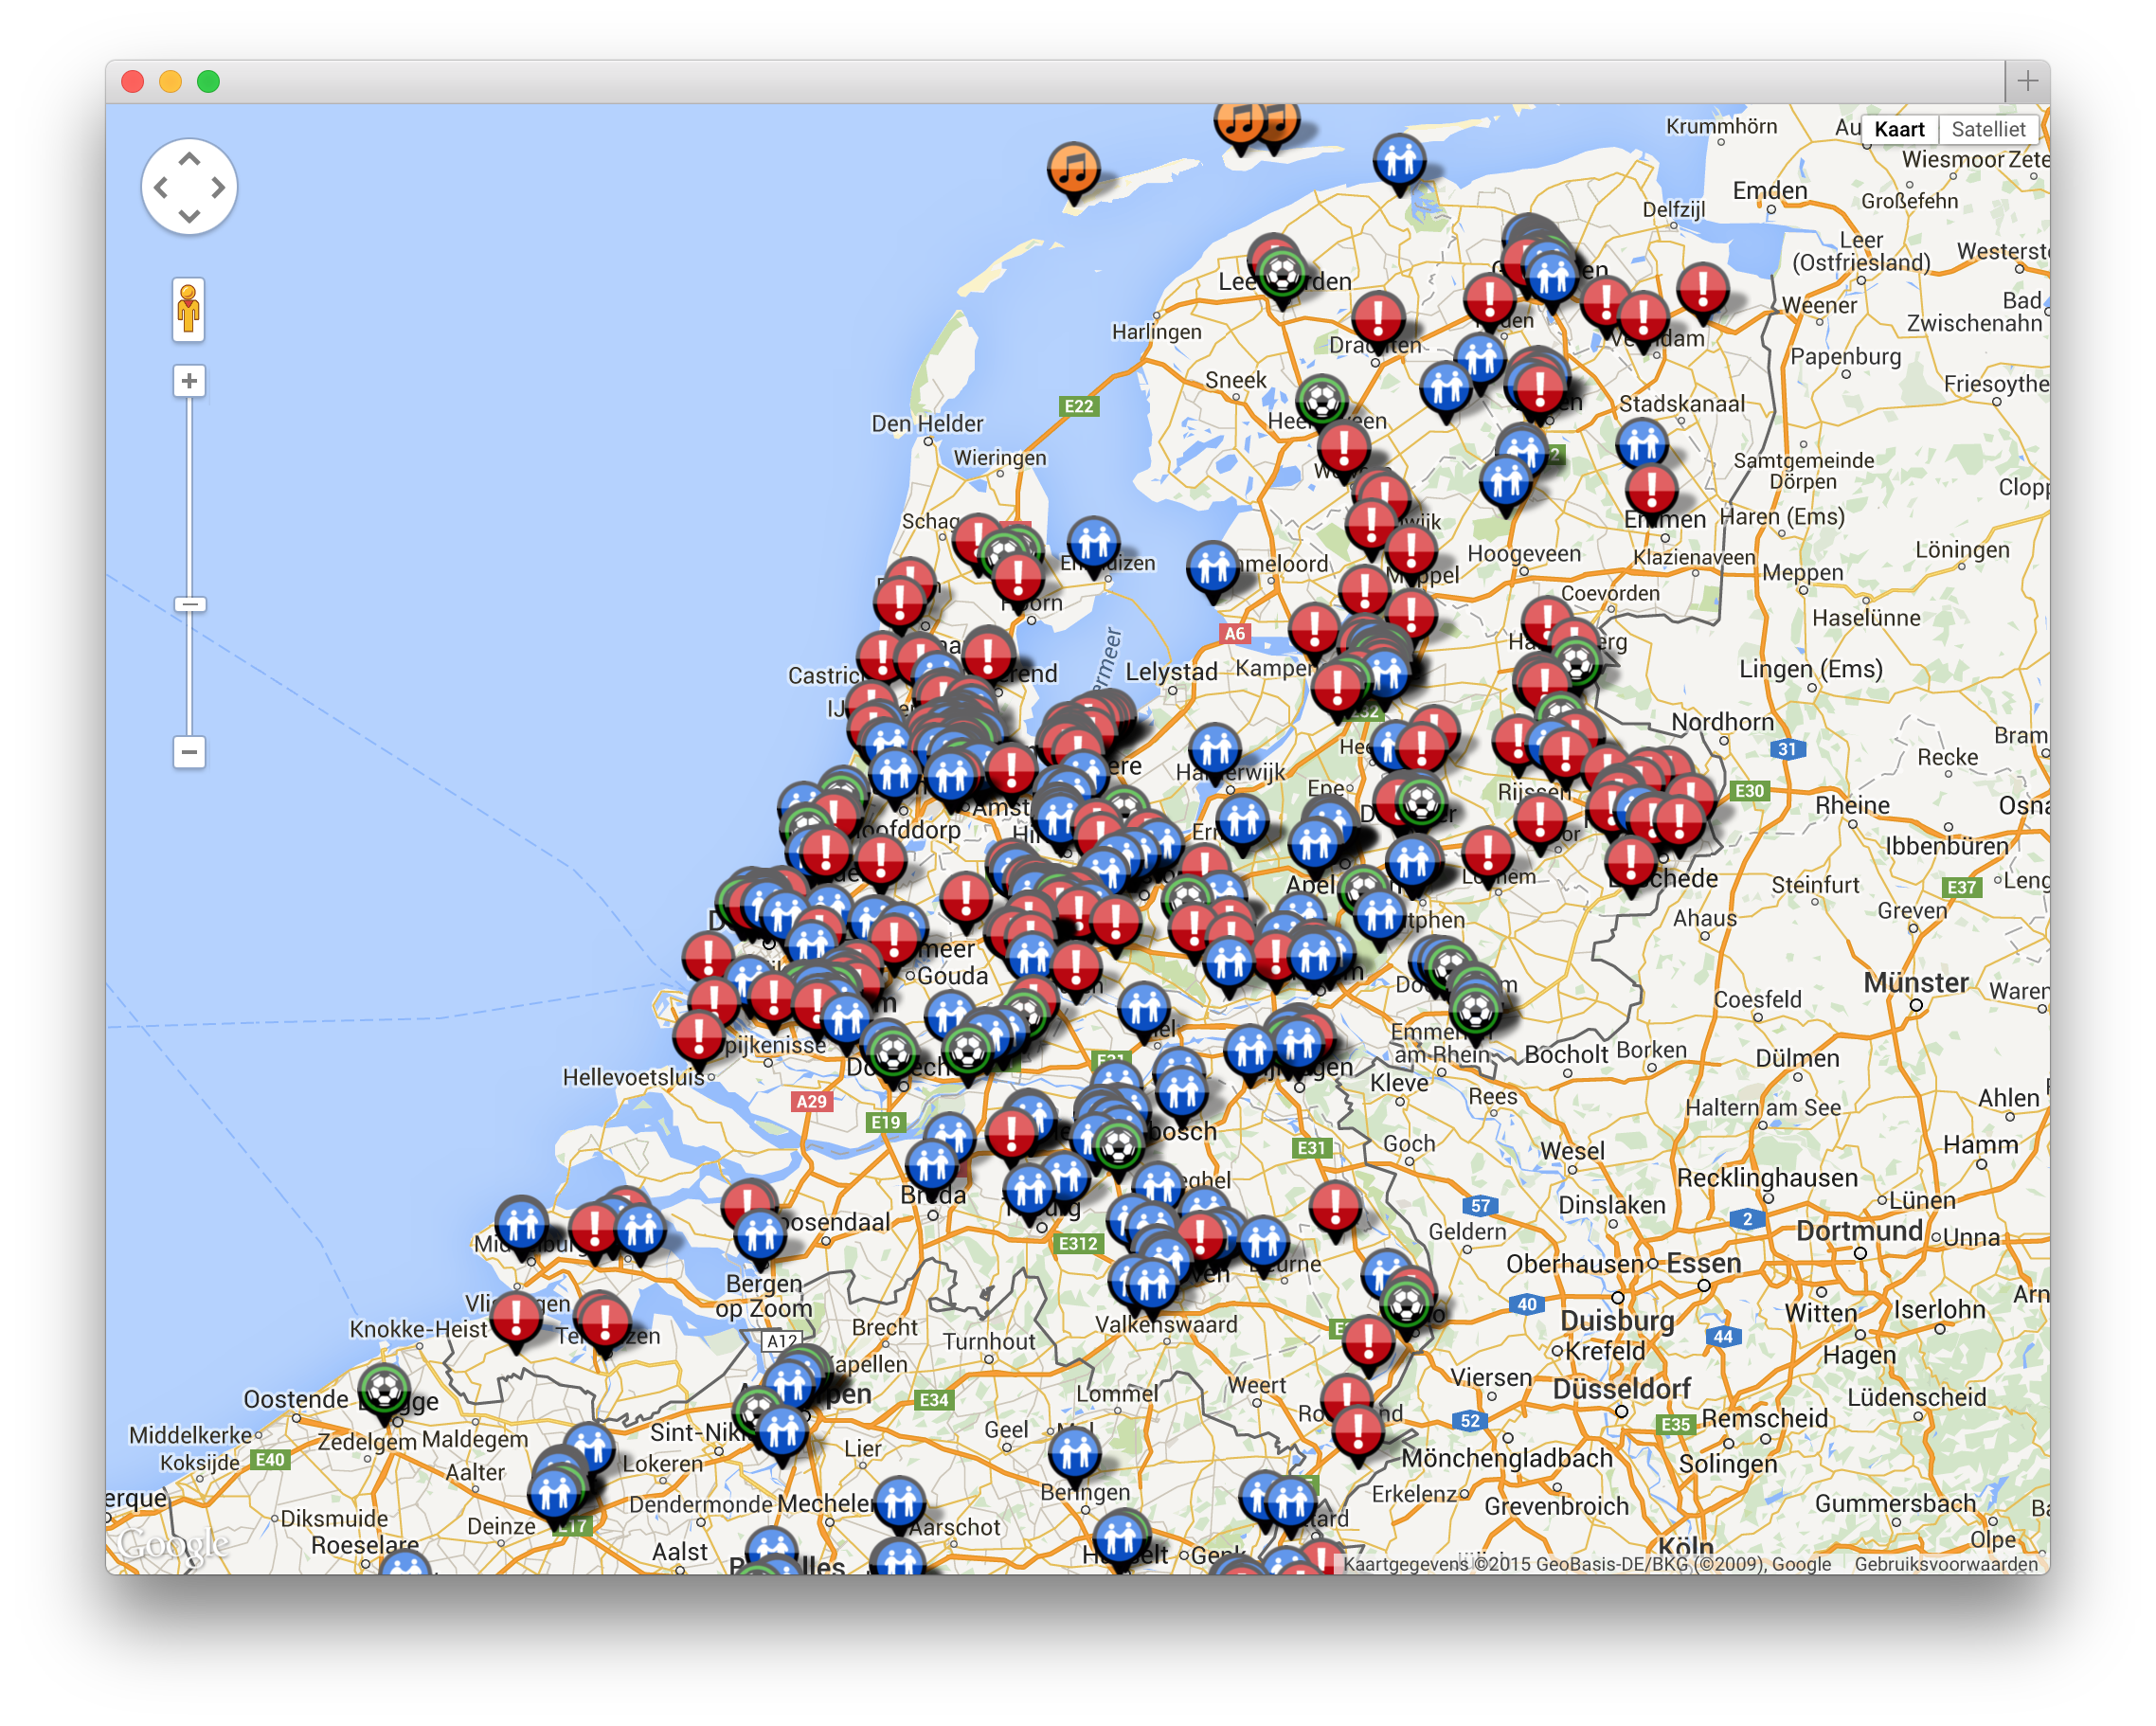
\includegraphics[width=4in]{voorkant.png} 
   \label{fig:gui}
\end{figure}


\subsection{Named Entity Recognition}
As discussed in chapters two and three a classifier was trained for detecting interesting entities within the events. The Stanford Named Entity software was used for this.

\subsubsection{Data collection}
For creating the silver standard I used the approach described in the previous chapter by first selecting lists of Dutch words for each category I want to recognize: locations, organizations, persons and miscellaneous.   I use the word lists that also are used in the Alpino software\footnote{Alpino is a dependency parser for Dutch, developed in the context of the PIONIER Project Algorithms for Linguistic Processing. } For each category I have a list of Dutch words related to that category. The wordlists are used to retrieve tweets that contain one or more of those words. 
\vl
I downloaded one million tweets and wrote a Python script to create the training file as can be seen in code example 11 that can be used to train your own classifier. In this example it shows that the training file is not perfect. The name \textit{van Zutphen} is a word in the person wordlist and thus is annotated as a name but in this case \textit{van} should not be annotated and \textit{Zutphen} should be annotated as a Location.

\begin{lstlisting}[language=Python, caption=Training file NER]
De 	 O
Sprinter 	 O
van 	 PERSON
Zutphen 	 PERSON
naar 	 O
Arnhem 	 LOCATION
van 	 O
00:06 	 O
vertrekt 	 O
van 	 O
spoor 	 O
1 	 O
Spoorwijziging 	 O
7690 	 O
\end{lstlisting}



\subsubsection{Training}
The training file (as can be seen in code example 7) was used to train the classifier. The documentation about the possible features was not so good and because the time it took to train the classifier (10 -14 hours) I could not experiment that much with different settings. I finally used the features also used for their standard classifier. That resulted in the results described in the next section. 

\subsubsection{Results}
The results can be found in table 7. The results show the difficulty of recognizing named entities in tweets and compared to other researches about named entity recognition the performance is not so high. \cite{ashwini2014targetable} conducted a research on finding what they call targetable named entities \textit{"named entities in a targeted set (e.g, movies, books, TV shows)"}, and can be compared to my system. Their resulting f-scores are between 76\% and 78\%.
\begin{table}[h]
 \centering
\caption[NER Classifier trained with Tweets]{NER Classifier trained with Tweets }
\begin{tabular}{|l|l|l|l|l|l|l|}
\hline
Entity       & P      & R      & F1     & TP & FP & FN   \\ \hline
LOCATION     & 0,7333 & 0,7333 & 0,7333 & 11 & 4  & 4    \\ \hline
MISC         & 0,0909 & 0,500  & 0,1538 & 1  & 10 & 1    \\ \hline
ORGANIZATION & 0,7500 & 0,8824 & 0,8108 & 15 & 5  & 2    \\ \hline
PERSON       & 0,6154 & 0,5517 & 0,5818 & 16 & 10 & 13   \\ \hline
Totals       & 0,5972 & 0,6825 & 0,6370 & 43 & 29 & 20 \\ \hline
\end{tabular}

\end{table}


\clearpage
\newpage
\section{Conclusion and discussion}
We are very pleased with the results of our classifier, compared to other researches our classifier performs very well and can be easily converted to a system that uses real-time tweets. Improvements could be to take a further look at our features and maybe think about tokenizing the tweet better. For example user names like \textit{@chrisPool} are detected by our system as \textit{chris Pool} but more difficult situations also occur like \textit{ArenA} and our system does not process that well. 
\vl
The named entity classifier results are a bit disappointing but it also shows how difficult the task is to recognize named entities in tweets. Because most classifiers do detection by looking at capitalized letters the classifier often tries to classify the wrong words. Improvements could also be to think about the automatic annotation of the training file. If a word occurs in more than one category list the system should use the most logical one. For example the case described in 4.7.1 data collection the location should have been the choice instead of person.
\vl
Looking back at my research questions I can say that is possible to detect and categorize local events in the Twitter stream using tweets with geo-information. Further analysis has to be done to find the optimal amount and types of  categories. Our system would make a nice website where people can see events in their neighborhood and filter categories they are interested in. Detecting the important entities is difficult, tweets are too short and noisy to detect entities. Improvements could be made by thinking about the processing of the tokens and to use the annotation by the user (\textit{Hashtag, emoticon})  more efficient. 


\newpage
\begin{landscape}
\section{Appendix 1}


\begin{table}[h]
 \centering
\begin{tabular}{|l|l|l|l|l|l|l|l|}
\hline
                          & accuracy & geen\_event    & sport          & entertainment  & bijeenkomst    & incident       & anders         \\ \hline
                          &          & P    R    F    & P    R    F    & P    R    F    & P    R    F    & P    R    F    & P    R    F    \\ \hline
All features              & 0.84     & 0.85 0.90 0.88 & 0.77 0.49 0.60 & 0.00 0.00 0.00 & 0.76 0.79 0.77 & 0.97 0.97 0.97 & 0.00 0.00 0.00 \\ \hline
Category                  & 0.81     & 0.85 0.82 0.84 & 0.73 0.46 0.56 & 0.00 0.00 0.00 & 0.66 0.84 0.74 & 0.99 0.97 0.98 & 0.00 0.00 0.00 \\ \hline
Location                  & 0.51     & 0.49 0.94 0.65 & 0.00 0.00 0.00 & 0.00 0.00 0.00 & 0.66 0.25 0.36 & 0.50 0.06 0.11 & 0.00 0.00 0.00 \\ \hline
WordOverlapSimple         & 0.63     & 0.60 0.85 0.71 & 0.00 0.00 0.00 & 0.00 0.00 0.00 & 0.57 0.33 0.42 & 0.77 0.83 0.80 & 0.00 0.00 0.00 \\ \hline
wordOverlapUser           & 0.6      & 0.57 0.93 0.71 & 0.00 0.00 0.00 & 0.00 0.00 0.00 & 0.00 0.00 0.00 & 0.66 0.90 0.76 & 0.00 0.00 0.00 \\ \hline
wordOverlapUser, category & 0.82     & 0.86 0.83 0.85 & 0.77 0.49 0.60 & 0.00 0.00 0.00 & 0.66 0.85 0.74 & 1.00 0.97 0.99 & 0.00 0.00 0.00 \\ \hline
\end{tabular}
\end{table}
\end{landscape}

\newpage
\section{Appendix 2}
\begin{table}[h]
 \centering
\caption[Confusion Matrix Naive Bayes]{Confusion Matrix Naive Bayes }
\begin{tabular}{|l|c|c|c|c|c|c|}
\hline
    & \multicolumn{1}{l|}{OTH} & \multicolumn{1}{l|}{MEE} & \multicolumn{1}{l|}{ENT} & \multicolumn{1}{l|}{NOE} & \multicolumn{1}{l|}{INC} & \multicolumn{1}{l|}{SPO} \\ \hline
OTH & \textless.\textgreater   & .                        & .                        & 1.                       & .                        & .                        \\ \hline
MEE & .                        & \textless82\textgreater  & 2                        & 14                       & .                        & 12                       \\ \hline
ENT & .                        & .                        & \textless.\textgreater   & 1                        & .                        & .                        \\ \hline
NOE & .                        & 27                       & 5                        & \textless179\textgreater & 1                        & 7                        \\ \hline
INC & .                        & .                        & .                        & 2                        & \textless76\textgreater  & .                        \\ \hline
SPO & .                        & 1                        & 1                        & 2                        & 1                        & \textless16\textgreater  \\ \hline
\end{tabular}
\end{table}
\begin{table}[h]
 \centering
\caption[Confusion Matrix Maximum Entropy]{Confusion Matrix Maximum Entropy }
\begin{tabular}{|l|c|c|c|c|c|c|}
\hline
    & \multicolumn{1}{l|}{OTH} & \multicolumn{1}{l|}{MEE} & \multicolumn{1}{l|}{ENT} & \multicolumn{1}{l|}{NOE} & \multicolumn{1}{l|}{INC} & \multicolumn{1}{l|}{SPO} \\ \hline
OTH & \textless.\textgreater   & 1                        & .                        & .                        & .                        & .                        \\ \hline
MEE & .                        & \textless81\textgreater  & 2                        & 7                        & 2                        & 11                       \\ \hline
ENT & .                        & .                        & \textless.\textgreater   & .                        & 1                        & .                        \\ \hline
NOE & .                        & 26                       & 5                        & \textless186\textgreater & 1                        & 7                        \\ \hline
INC & .                        & 1                        & .                        & 4                        & \textless73\textgreater  & .                        \\ \hline
SPO & .                        & 1                        & 1                        & 2                        & 1                        & \textless16\textgreater  \\ \hline
\end{tabular}
\end{table}
\begin{table}[h]
 \centering
\caption[Confusion Matrix SVM classifier]{Confusion Matrix SVM classifier }
\begin{tabular}{|l|c|c|c|c|c|c|}
\hline
    & \multicolumn{1}{l|}{OTH} & \multicolumn{1}{l|}{MEE} & \multicolumn{1}{l|}{ENT} & \multicolumn{1}{l|}{NOE} & \multicolumn{1}{l|}{INC} & \multicolumn{1}{l|}{SPO} \\ \hline
OTH & \textless.\textgreater   & 1                        & .                        & .                        & .                        & .                        \\ \hline
MEE & .                        & \textless89\textgreater  & 2                        & 31                       &                          & 14                       \\ \hline
ENT & .                        & .                        & \textless.\textgreater   & .                        &                          & .                        \\ \hline
NOE & .                        & 19                       & 5                        & \textless166\textgreater & 1                        & 4                        \\ \hline
INC & .                        & .                        & .                        & .                        & \textless73\textgreater  & .                        \\ \hline
SPO & .                        & 1                        & 1                        & 2                        & 1                        & \textless17\textgreater  \\ \hline
\end{tabular}

\end{table}

%----------------------------------------------------------------------------------------
\newpage
\bibliographystyle{authordate1}
\bibliography{chris}
\end{document}